\documentclass[10pt,aspectratio=1610]{beamer}

\usetheme[progressbar=frametitle,sectionpage=none,background=light]{metropolis}

%%––––––––––––––––––––––––––––––––––––––––––––––––
% Define styles
%%––––––––––––––––––––––––––––––––––––––––––––––––

%%––––––––––––––––––––––––––––––––––––––––––––––––
% Setting up colors
\definecolor{logoblue1}{RGB}{35, 121, 181}
\definecolor{logoblue2}{RGB}{88, 145, 202}
\definecolor{darkblue}{RGB}{25, 41, 54}
\definecolor{lightgrey}{RGB}{134, 143, 161}
\definecolor{greytext}{RGB}{102, 118, 128}
\definecolor{darktext}{RGB}{29, 43, 52}
\definecolor{green}{RGB}{0, 184, 44}
\definecolor{vividblue}{RGB}{15, 117, 183}
\definecolor{orange}{RGB}{246, 177, 70}
\definecolor{lightblue}{RGB}{244, 247, 251}
\definecolor{white}{RGB}{255, 255, 255}
\definecolor{red}{RGB}{183, 25, 29}

\setbeamercolor{frametitle}{bg=darkblue, fg=lightblue}
\setbeamercolor{background canvas}{bg=black}
\setbeamercolor{normal text}{fg=lightblue}
%%––––––––––––––––––––––––––––––––––––––––––––––––

%%––––––––––––––––––––––––––––––––––––––––––––––––
% Setting up fonts
\usepackage{lato}
\usepackage{roboto}
\usepackage{montserrat}

\setbeamerfont{frametitle}{family=\flafamily, size*={18}{18}}
% \setbeamerfont{footline}{family=\fontfamily{montserrat}}
% \setbeamerfont{normal text}{family=\roboto, size*={16}{18}}

% Setting up fonts for bibliography style
\setbeamerfont{bibliography entry author}{size=\small}
\setbeamerfont{bibliography entry title}{size=\small}
\setbeamerfont{bibliography entry location}{size=\small}
\setbeamerfont{bibliography entry note}{size=\small}
\setbeamerfont{bibliography item}{size=\small}
%%––––––––––––––––––––––––––––––––––––––––––––––––

\usepackage{appendixnumberbeamer}

\usepackage{booktabs}
\usepackage[scale=2]{ccicons}

\usepackage{pgfplots}
\usepgfplotslibrary{dateplot}

\usepackage{xspace}
\newcommand{\themename}{\textbf{\textsc{metropolis}}\xspace}

\usepackage{hyperref}
\hypersetup{
  colorlinks, 
  urlcolor=vividblue, 
  citecolor=lightblue, 
  linkcolor=lightblue
}

\setbeamertemplate{frame footer}{{\large\textcolor{logoblue1}{source}\textcolor{logoblue2}{\{d\}}}}


\title{Exploratory code search and snippet suggestion}
\subtitle{Article review}
\date{\today}
\author{Slavnov Konstantin\\konstantin@sourced.tech}
%\titlegraphic{\hfill
\includegraphics[height=1.5cm]{logo.png}}

\begin{document}

\maketitle

\section{Introduction}

  

\begin{frame}[fragile]{Introduction}

  What is the \textbf{fastest} way to learn a new library? 

  New framework investigation ways:
  \begin{itemize}
    \item Documentation reading;
    \item Ask stackoverflow;
    \item \alert<2>{Just start to use it;}
    \item \alert<2>{Search code examples;}
    \item etc
  \end{itemize}

  \vfill
  \pause
  \textbf{Insights} from Searching and Skimming: An Exploratory Study \cite{starke2009searching}.

\end{frame}
\begin{frame}[fragile]{Ways to solve}
  Let's build a machine learning assistant! 

  Approaches:
  \begin{itemize}
    \item \alert<2>{Topic modeling}
    \item Hierarchical clustering
    \item Deep learning way
    \item Probabilistic way
  \end{itemize}
\end{frame}


\section{Approaches}

\begin{frame}{Topic modeling}
  Scheme
  \begin{itemize}
    \item Get a codebase of library usage
    \item Build a hierarchical topic modeling for codebase
    \item Show it for user API query
    \item ???
    \item PROFIT!
  \end{itemize}
\end{frame}

\begin{frame}{Flat topic model. Reminder}
  \begin{itemize}
    \item Documents $d \in D$
    \item Tokens (words) $w \in W$
    \item Topics $t \in T$
    \item Document-token counters $n_{dw}$\\[3mm]
  \end{itemize}
  Flat topic model:\\[-1mm]
  $$
    P_{wd} = \dfrac{n_{dw}}{\sum_{w' \in W} n_{dw'}} = p(w \mid d) \approx \sum_{t \in T} p(w \mid t)\, p(t \mid d) = \sum_{tin} \phi_{wt} \theta_{td} = \{\Phi \Theta\}_{wd}
  $$
  or just
  $$
      P \approx \Phi \Theta
  $$
  \pause
  Applying MLE:
  $$
    L(\Psi, \Theta) = \sum_{d\in D}
      \sum_{w \in d} n_{dw} \ln 
        \sum_t \psi_{wt} \theta_{td} \quad
    \longrightarrow \max_{\Psi, \Theta \text{ -- stochastic}}
  $$

  EM-algorithm is used for training.
\end{frame}

\begin{frame}{Flat topic model.}

   \href{http://bigartm.org}{BigARTM} is good tool for it.

  What we can do:
  \begin{itemize}
    \item Add regularisers: \quad 
      $$ L(\Psi, \Theta) + R(\Psi, \Theta) 
         \longrightarrow \max $$
    \item Add modalities $m \in M$. 
      $$W = \bigsqcup_{m \in M} W_m  \text{ and } \Phi = [\Phi_1 | \cdots | \Phi_n ]$$
  \end{itemize}
  \vspace{5mm}
  \pause
  Let's build \textbf{topic hierarchies}.
  \begin{itemize}
    \item Each level is a topic model.
    \item Next level is learned with \textbf{specific regulariser} to find
parent topics from previous level.
  \end{itemize}
  \vspace{5mm}
  Check out \cite{vorontsov2014additive, vorontsov2014tutorial}.
\end{frame}

\begin{frame}{Topic hierarchies.}
  \begin{itemize}
  \item \textbf{Learned} parent level: topics $a \in A$ with $\Phi' \in \mathbb{R}^{|W| \times |A|} $ and $\Theta' \in \mathbb{R}^{|A| \times |D|} $.
  \item \textbf{To learn:} \\
      \quad New level with topics $t \in T$ and $\Phi \in \mathbb{R}^{|W| \times |T|} $ and $\Theta \in \mathbb{R}^{|T| \times |D|} $.\\
      \quad Parent-child relations $\Psi_{ta}$  -- $t$ is a child of $a$.
  \pause
  \item \textbf{Assumption:} parent topic is a mixture of children's: \\[2mm]
  \qquad\qquad
  $\displaystyle
      p(w \mid a) \approx \sum_{t \in T} \; p(w \mid t) p(t \mid a)
  $
  \qquad or just \qquad
  $
    \Phi^l \approx  \Phi \Psi
  $
  \pause
  \item We can just add $|A|$ pseudo documents with $n_{wa}$ counters
  \pause
  \item The same point with $\Theta$ regularisation.
  $
  \Theta^l \approx \tilde \Psi \Theta
  $
  It is like add new modality with tokens corresponding to $a \in A$.
  \end{itemize}

\end{frame}

\begin{frame}{Hierarchy sparsing}
  \textbf{The goal:}\quad Topics should have small number of parents. \\[5mm]

  $p(a \mid t)$ should be sparse.
  
  Similar to LDA regulariser:
  $$
      R(\Psi) 
        = \dfrac{1}{|A|} \sum_a \sum_t \ln p(a \mid t)
        = \dfrac{1}{|A|} \sum_a \sum_t \ln 
            \dfrac{\psi_{ta} \; p(a)}{\sum_{a'} \psi_{ta'} \; p(a')}
  $$

  To apply we need just to update M-step of EM-algorithm.

  The same approach for $\Theta$ regularisation.
\end{frame}

\begin{frame}{Hierarchical clustering approach}
  Scheme
  \begin{itemize}
    \item Get a codebase of library usage
    \item \alert<2>{Somehow get a document representations in $\mathbb{R}^{d}$}
    \item Build a hierarchical clusterization
    \item Show it for user API query
    \item ???
    \item PROFIT!
  \end{itemize}
\end{frame}

\begin{frame}{DocNADE}
  \begin{columns}[T,onlytextwidth]
    \column{0.7\textwidth}
      \textbf{NADE} -- Neural Autoregressive Distribution Estimator \cite{larochelle2011neural}.\\[2mm]

      Based on fact that \qquad
      $ \displaystyle
        p(v) = 
          \prod_{d=1}^D p(v_d \mid v_{<d})
      $ \\[3mm]
      We need to \textbf{parametrise} $p(v_d \mid v_{<d})$.\\[-3.5mm]
      \pause
      $$
        p(v_d \mid v_{<d}) = \mathrm{sigm}(b_d + V_{d,:}h_d)
      $$
      $$
        h_d = \mathrm{sigm}(c + W_{:, <d}v_{<d}).
      $$

      $W, V, b, c$ -- learnable parameters by LME.
      \pause
      Softmax is used for vectors modeling:
      $$
        p(v_d \mid v) = \dfrac{\exp(b_{w_b} + V_{w_d, :}h_d)}{\sum_w\exp(b_{w} + V_{w, :}h_d)}
      $$
      \pause
      Trains on random permutations of the words in a document.

    \column{0.4\textwidth}
      \vspace{7mm}
      \quad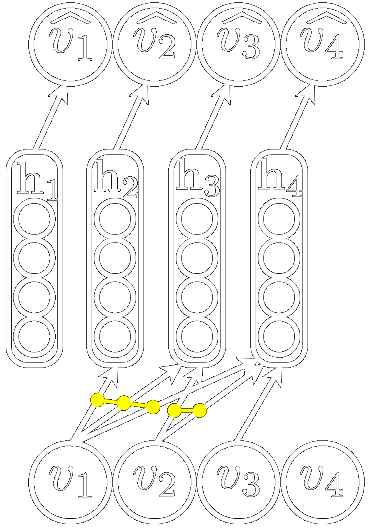
\includegraphics[width=4.2cm]{./imgs/nade.png}
  \end{columns}
  Document representation is $h_T$ at the final timestep $T$.
\end{frame}

\begin{frame}{Deep learning way}
  \begin{itemize}
    \item  \textbf{Aim:} Generate API sequences for a natural language query \cite{gu2016deepAPILearning}.
    \item  \textbf{Method:} RNN encoder-decoder model for API learning.
    \item  \textbf{Data:} annotated code snippets collected from GitHub.
  \end{itemize}
  \centering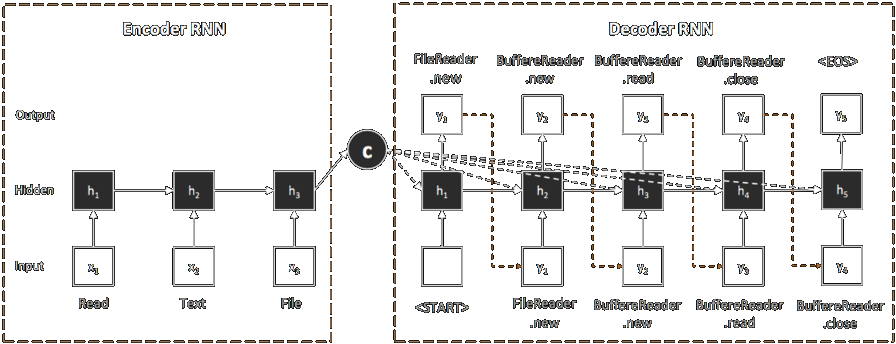
\includegraphics[width=12cm]{./imgs/rnn-encoder-decoder.png}
\end{frame}

\begin{frame}{Deep learning way}
  \textbf{Details:} 
  \begin{itemize}
    \item Run on sequences of API methods only.
    \item RNN is \textbf{GRU}, Encoder is bidirectional with attention, 1000 hidden units, 120 dimension of word embeddings.
    \item Beam Search for generation several API sequences to choose
    \pause
    \item IDF-based weights for API as a penalty term in \textbf{loss}:
    $$
      \mathrm{loss}_{it} = - \log p_\theta (y_{it} \mid x_i) - \lambda \log(\dfrac{N}{n_{t}})
    $$
    where\\
    \quad $i$ is $i$-th train instance,\\
    \quad $t$ is $t$-th target word in instance i,\\
    \quad $N$ is the total number of API sequences,\\
    \quad $n_t$ is the number of sequences where the API $t$ appears.\\

  \end{itemize}
\end{frame}

\begin{frame}{Probabilistic way. Interesting Sequence Mining}
  \begin{columns}[T,onlytextwidth]
  \column{0.55\textwidth}
      \textbf{Task:} get meaningful API patterns $\mathcal{I}$ \cite{fowkes2016ProbabilisticAPIMining, fowkes2016subsequenceMining}.\\[2mm]

      \textbf{Idea:} Use API patterns $\mathcal{I}$ to define a code probability in database $X$.\\[2mm]

      Pattern is interesting code \textbf{subsequence}.\\[2mm]
      \pause
      Simplified model:
      $$
          p(X, z \mid \mathcal{I}) \sim \prod_{i \in \mathcal{I}\cap X} p_i^{z_i} (1 - p_i)^{1-z_i}
      $$

      \vspace{3mm}

      {\small
      $X$ -- code database,

      $\mathcal{I}$ -- set of API patterns,

      $p_i$ -- API pattern $i \in \mathcal{I}$ probability,

      $z_i$ -- indicator of including pattern into code (hidden).
      }
      \pause
  \column{0.03\textwidth}
  \column{0.03\textwidth}
  Example:\\[2mm]
  \column{0.35\textwidth}
  \vspace{3mm}

    \setlength{\tabcolsep}{2pt}
    \begin{tabular}{llllllll}
               &   &   &   &   &   &    &     \\
      $X =$ \{ & d & b & c & e & d & f  & f;   \\
               & e & e & d & f & f & f; &     \\
               & d & f & d & e & f & f; & \}  
    \end{tabular}
    
    \vspace{5mm}

    \begin{tabular}{lccccc}
      $\mathcal{I} =$ \{ & [ b c e ] & [ d f ] & [ d f ] & [ e f ] &\}\\[2mm]
                         &     1     &    1    &    1    &    0    &  \\
            $z:$         &     0     &    1    &    0    &    1    &  \\
                         &     0     &    1    &    1    &    1    &  \\[2mm] 
            $p_i:$       &    0.33   &    1    &   0.66  &   0.66  &  \\

    \end{tabular}
  \end{columns}
\end{frame}

\begin{frame}{Probabilistic way. Interesting Sequence Mining}
  \begin{columns}[T,onlytextwidth]
  \column{0.55\textwidth}
   \textbf{Solver:} EM-algorithm.

   Iterate:
   \begin{enumerate}
      \item Structural-EM ($\mathcal{I}$ update)
      \begin{enumerate}
        \item Somehow generate candidate $S'$ 
        \item See if quality increases
      \end{enumerate} 
      \item Hard-EM ($z$ and $p$ update)
        \begin{enumerate}
          \item Find patterns from $\mathcal{I}$ that was used to sample $X$ with greedy search.
          $$
            z = \arg\max_z \log p(z \mid p, \mathcal{I}; X)
          $$ 
          \item Update $p_i$ by averaging $z$.
        \end{enumerate}
  \end{enumerate}
  \column{0.03\textwidth}
  \column{0.03\textwidth}
  Example:\\[2mm]
  \column{0.35\textwidth}
  \vspace{3mm}

    \setlength{\tabcolsep}{2pt}
    \begin{tabular}{llllllll}
               &   &   &   &   &   &    &     \\
      $X =$ \{ & d & b & c & e & d & f  & f;   \\
               & e & e & d & f & f & f; &     \\
               & d & f & d & e & f & f; & \}  
    \end{tabular}
    
    \vspace{5mm}

    \begin{tabular}{lccccc}
      $\mathcal{I} =$ \{ & [ b c e ] & [ d f ] & [ d f ] & [ e f ] &\}\\[2mm]
                         &     1     &    1    &    1    &    0    &  \\
            $z:$         &     0     &    1    &    0    &    1    &  \\
                         &     0     &    1    &    1    &    1    &  \\[2mm] 
            $p_i:$       &     0.33  &    1    &   0.66  &   0.66  &  \\

    \end{tabular}
\end{columns}
\end{frame}

\begin{frame}{References. Links}
  \begin{enumerate}
    \item \href{http://www.machinelearning.ru/wiki/images/d/dc/2.Chirkova.pdf}{Hierarchical Multimodal Topic Modeling presentation. N. A. Chirkova and K. V. Vorontsov}
    \item \href{http://bigartm.org}{BigARTM for Topic Modeling}
    \item \href{http://blog.aylien.com/tensorflow-implementation-neural-autoregressive-topic-model-docnade/}{Post about DocNADE with implementation}
    \item \href{https://github.com/mast-group/api-mining}{Probabilistic API Mining code}


  \end{enumerate}

\end{frame}

\begin{frame}[allowframebreaks]{References. Articles}

  \setbeamertemplate{bibliography item}{\insertbiblabel}
  \bibliography{bibl.bib}
  \bibliographystyle{abbrv}

\end{frame}

\end{document}
